\chapter{Formulating a Mathematical Model}
based on DAE lecture and \cite{ModellingAndDiscretizationOfCircuitProblems}

To accurately represent a physical system in a mathematical model we first have to think about \textbf{how} to best formulate a mathematical model that formulates this system accurately enough.
This chapter aims to elaborate on the Modified Nodal Analysis (MNA) of an electrical circuit, which is the a common choice for these kinds of models. For this we have to introduce the notions of network topology as well as some basic electrical components and laws. Most of the following notions such as voltage, current and electrical potentials are time dependent. For better readability we will leave out the time argument $t$ in some cases.

\section{Network Topology}
\label{Sec:Network Topology}
An electrical circuit is usually considered as a graph $(\mathcal{N},\mathcal{E})$ where $\mathcal{N} = (n_0, n_1, n_2, ..., n_k)$ denotes nodes and $\mathcal{E} = \{e_{j}: j = 1,...,l\}$ is the set of edges where $|\mathcal{N}| = k$ is the number of nodes and $|\mathcal{E}| = l$ the number of edges. If for some $i$ and some $j$ the nodes $n_i$ and  $n_j$ are connected, then there exists an edge connecting those two nodes.
We can store this information in an \emph{incidence matrix} $\tilde{A} = (\tilde{a}_{ij}) \in \mathbb{R}^{k \times l}$ which is defined by
\begin{displaymath}
	\tilde{a}_{ij} = 
	\begin{cases}
		1 &   \text{edge $j$ starts at node $i$},\\
		-1 &  \text{edge $j$  ends at node $i$},\\
		0 & \text{else}.				
	\end{cases}
\end{displaymath}
We call $u = (u_0, u_1, u_2, ...)$ the corresponding electrical potentials (or just potentials) to the nodes $\mathcal{N}$. The difference between the potentials at two connected nodes is called the voltage at the respective edge. To fix the absolute values of these potentials we have to set one node to a fixed value. We will do that by ``grounding'' the node $n_0$, which means we set the potential $u_0 = 0$. The grounding of a node allows us to remove the corresponding row from the incidence matrix to get the \emph{reduced incidence matrix} $A$. The vector $v = (v_{ij})_{ij}$ represents the voltages at the edges. For some $i$ and some $j$ the voltage at edge $ij$ is $v_{ij} = u_i - u_j$.

We will later see, that the components of an electrical circuit, which will be installed along the edges, describe a relationship between the current along the edge the corresponding voltage. Thus a current vector $i = (i_1, i_2, i_3, ...)$ containing the currents along the edges is required.


\textbf{Example 1} \label{ex:network topology} \\
As an example we consider the charging of a capacitor. The circuit is given as
\begin{figure}[H]
	\label{circuit:charging of capacitor}
	\centering
	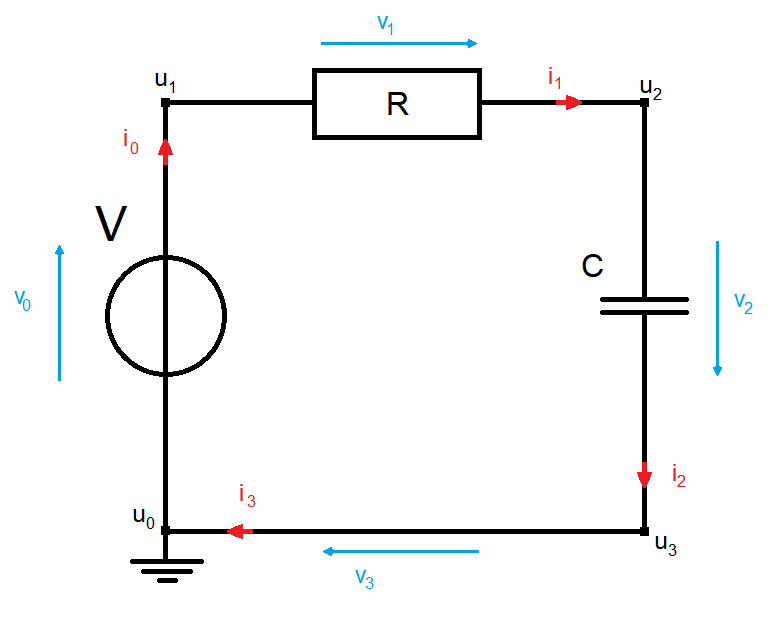
\includegraphics[scale=0.5]{pictures/Example1_simple.png}
	\caption{charging capacitor with series resistor and voltage source}
\end{figure}
with the node-potentials, the voltages and the currents collected in the vectors
\begin{displaymath}
	u=
	\left(
	\begin{matrix}
		u_0 \\
		u_1 \\
		u_2 \\
		u_3 
	\end{matrix}
	\right),
	\quad
	v=
	\left(
	\begin{matrix}
		v_0 \\
		v_1 \\
		v_2 \\
		v_3 
	\end{matrix}
	\right),
	\quad
	i=
	\left(
	\begin{matrix}
		i_0 \\
		i_1 \\
		i_2 \\
		i_3 
	\end{matrix}
	\right).
\end{displaymath}
The incidence matrix of this circuit has the form
\begin{displaymath}
	\tilde{A} = 
	\left(
	\begin{matrix}
		1 & 0 & 0 & -1 \\
		-1 & 1 & 0 & 0 \\
		0 & -1 & 1 & 0 \\
		0 & 0 & -1 & 1 
	\end{matrix}
	\right).
\end{displaymath}
The rows of this matric correspond to the nodes of the circuit and the columns correspond to the edges. By grounding node 0 this reduces to
\begin{displaymath}
	A = 
	\left(
	\begin{matrix}
		-1 & 1 & 0 & 0 \\
		0 & -1 & 1 & 0 \\
		0 & 0 & -1 & 1 
	\end{matrix}
	\right).
\end{displaymath}
In this circuit edge 3 is not populated with any components. This means that the voltage along this edge does not change, or in terms of potentials
\begin{displaymath}
	u_0 - u_3 = 0.
\end{displaymath}
Thus we can consider this circuit with node 0 and node 3 merged. This leads to a slightly different incidence and reduced incidence matrix, i.e.
\begin{displaymath}
	\tilde{A} = 
	\left(
	\begin{matrix}
		1 & 0 & -1 \\
		-1 & 1 & 0 \\
		0 & -1 & 1 \\
	\end{matrix}
	\right) \quad \text{and} \quad
	A = 
	\left(
	\begin{matrix}
		-1 & 1 & 0 \\
		0 & -1 & 1 
	\end{matrix}
	\right), \quad \text{respectively.}
\end{displaymath}


\textbf{Example 2} \label{ex:LC-circuit incidence matrix} \\
Another example is the a circuit that only contains a capacitor and an inductor. This circuit will oscillate, if given appropriate initial conditions.
\begin{figure}[H]
	\label{circuit:LC-circuit}
	\centering
	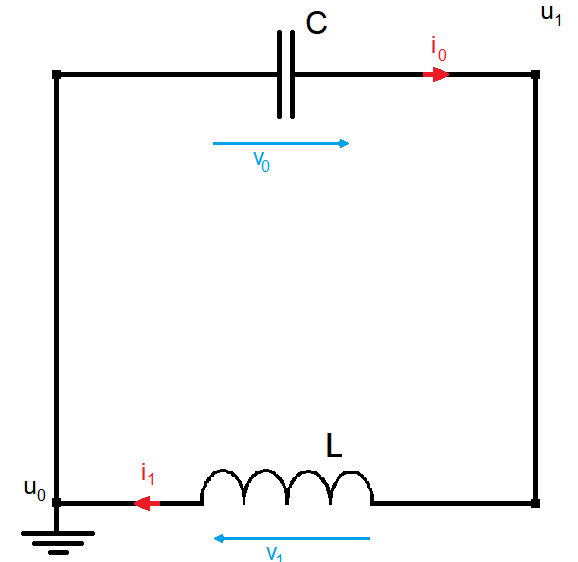
\includegraphics[scale=0.5]{pictures/Example2_index0.png}
	\caption{capacitor and inductor oscillator}
\end{figure}

we again collect the node-potentials, the voltages and the currents in the vectors
\begin{displaymath}
	u=
	\left(
	\begin{matrix}
		u_0 \\
		u_1
	\end{matrix}
	\right),
	\quad
	v=
	\left(
	\begin{matrix}
		v_0 \\
		v_1
	\end{matrix}
	\right),
	\quad
	i=
	\left(
	\begin{matrix}
		i_0 \\
		i_1
	\end{matrix}
	\right).
\end{displaymath}
The incidence matrix of this circuit has the form
\begin{displaymath}
	\tilde{A} = 
	\left(
	\begin{matrix}
		1 & -1  \\
		-1 & 1 
	\end{matrix}
	\right).
\end{displaymath}
The rows of this matric correspond to the nodes of the circuit and the columns correspond to the edges. By grounding node 0 this reduces to
\begin{displaymath}
	A = 
	\left(
	\begin{matrix}
		-1 & 1  
	\end{matrix}
	\right).
\end{displaymath}


\textbf{Example 3} \label{ex:Example 3 - incidence matrix } \\
As a third example we consider a similar circuit to the circuit presented in \ref{ex:network topology}, the only difference is that we connected the resistor parallel to the capacitor instead of in series.
\begin{figure}[H]
	\label{circuit:Example 3}
	\centering
	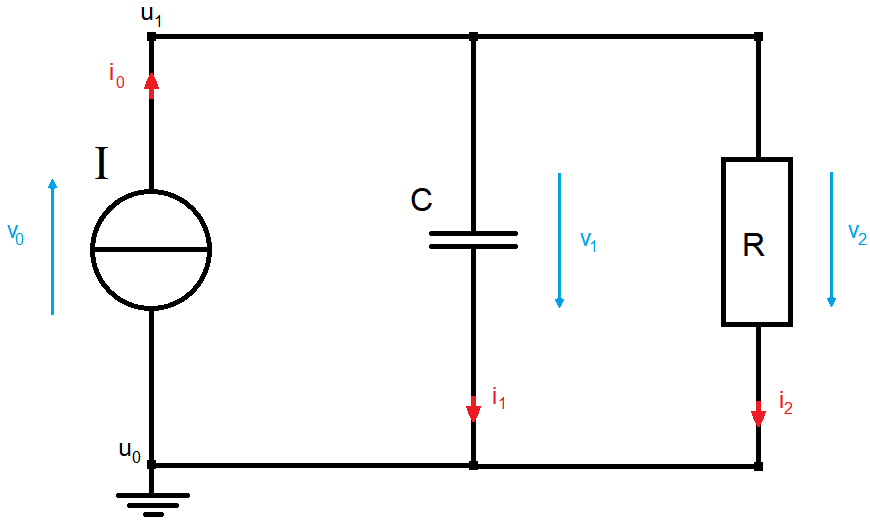
\includegraphics[scale=0.5]{pictures/Example3.png}
	\caption{Capacitor with resistor and voltage source}
\end{figure}

We collect the node-potentials, the voltages and the currents collected in the vectors
\begin{displaymath}
	u=
	\left(
	\begin{matrix}
		u_0 \\
		u_1 
	\end{matrix}
	\right),
	\quad
	v=
	\left(
	\begin{matrix}
		v_0 \\
		v_1 \\
		v_2 
	\end{matrix}
	\right),
	\quad
	i=
	\left(
	\begin{matrix}
		i_0 \\
		i_1 \\
		i_2 
	\end{matrix}
	\right).
\end{displaymath}
The incidence matrix of this circuit has the form

\begin{displaymath}
	\tilde{A} = 
	\left(
	\begin{matrix}
		1 & -1 & -1 \\
		-1 & 1 & 1 
	\end{matrix}
	\right),
\end{displaymath}
this leads to the reduced incidence matrix
\begin{displaymath}
	A = 
	\left(
	\begin{matrix}
		-1 & 1 & 1
	\end{matrix}
	\right).
\end{displaymath}



\section{Energy Conservation Laws}
To fully fix all the variables that arise in the model of an electrical circuit we will need some \emph{conservation laws}. In this context, conservation laws are a description of physical properties that can be observed in electrical circuits. This means that they have to be fulfilled non the less, thus including them into the system also makes sense from a physical perspective. 
\begin{itemize}
	\item \textbf{Kirchhoff's voltage law (KVL):} \newline
	The sum of voltages along each loop of the network must equal to zero. Using the incidence matrix $A$ this law can be formulated as
	\begin{equation}
		\label{KVL}
		A^\top  u = v.
	\end{equation}
	\item \textbf{Kirchhoff's current law (KCL):} \newline
	For any node, the sum of currents flowing into the node is equal to the sum of currents flowing out of the node. Using the incidence matrix $A$ again, this law can be formulated as
	\begin{equation}
		\label{KCL}
		A  i = 0.
	\end{equation}
\end{itemize}

\section{Electrical Components and their relations}
\label{Sec:Electrical Components and their relations}
Electrical components are described by equations relating their edge voltage $v$ to their edge current $i$. We will mainly focus on so-called RLC-networks (short for Resistor, Inductor, Capacitor), which consist of resistors, capacitors, inductors, voltage sources and current sources. Diodes and transistors as well as other electrical components can be described in a similar way, although these lead to a more difficult analysis of the system, see e.g. \cite{ModellingAndDiscretizationOfCircuitProblems} and \cite{SchwarzTischendorfCircuitMNA}. Using the notation introduced in Section \ref{Sec:Network Topology}, the relations read as:
\begin{itemize}
	\item \textbf{Resistor} \newline
	Resistors ''resist`` the flow of current, which causes voltage to drop. This behaviour is described by the \emph{resistance} $R \in \mathbb{R}^+ := \{x \in \mathbb{R}: x > 0\}$ which is given in \emph{Ohm} ($\Omega$) and its reciprocal, the \emph{conductance} $G \in \mathbb{R}^+$, which is given in \emph{Siemens} ($S=\frac{1}{\Omega}$). 
	\begin{equation}
		\label{eq:resistor law}
		v = R \ i \quad \text{or} \quad i = G \ u.
	\end{equation}
	\begin{figure}[H]
		\label{fig:resistor symbol}
		\centering
		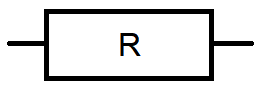
\includegraphics[width=2cm]{pictures/resistor.png}
		\caption{resistor symbol}
	\end{figure}

	\item \textbf{Capacitor} \newline
	Capacitors ''store`` electrical energy by accumulating electrical charge. Their characteristic equations can be described directly using the stored charge $Q \in \mathbb{R}^+_0 := \{x \in \mathbb{R}: x \geq 0\}$ or indirectly using the change in charge, which is nothing other than the current $I$. The \emph{capacitance} $C \in \mathbb{R}^+$ is given in \emph{Farads} ($F$).
	\begin{equation}
		\label{eq:capacitor law}
		Q = C \ v \quad \text{and by derivation in t} \quad I = C \ \frac{d}{dt}v = C \ v'.
	\end{equation}
	\begin{figure}[H]
		\label{fig:capacitor symbol}
		\centering
		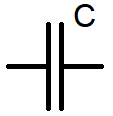
\includegraphics[width=2cm]{pictures/capacitor.png}
		\caption{capacitor symbol}
	\end{figure}

	\item \textbf{Inductor (Coil)} \newline
	An electric current flowing through a conductor generates a magnetic field $\Phi \in \mathbb{R}^{n \times n}$ surrounding it. This magnetic field causes a voltage drop dependant on the change in current. The \emph{inductance} $L \in \mathbb{R}^+$ is given in \emph{Henry} ($H$).
	\begin{equation}
		\label{eq:inductor law}
		\Phi = L \ i \quad \text{and by derivation in t} \quad v = L \ i'.
	\end{equation}
	\begin{figure}[H]
		\label{fig:inductor symbol}
		\centering
		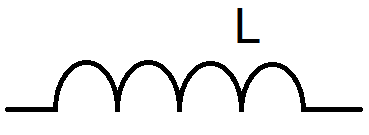
\includegraphics[width=3cm]{pictures/inductance.png}
		\caption{inductor symbol}
	\end{figure}

	\item \textbf{Voltage Source} \newline
	A voltage source supplies the system with a voltage. It can either supply varying amounts of voltage (with the special case of alternating current AC) or a fixed amount of voltage. The unit of voltage is \emph{Volts} ($V$).
	\begin{equation}
		\label{eq:voltage source law}
		v = v_{src}
	\end{equation}
	\begin{figure}[H]
		\label{fig:voltage source symbol}
		\centering
		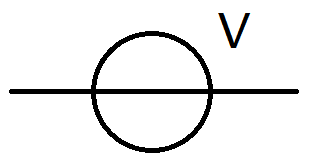
\includegraphics[width=4cm]{pictures/voltage_source.png}
		\caption{voltage source symbol}
	\end{figure}

	\item \textbf{Current Source} \newline
	A current source supplies the system with current. It can either supply varying amounts of current (with the special case of alternating current AC) or a fixed amount of current. The unit of current is \emph{Ampere} ($A$).
	\begin{equation}
		\label{eq:current source law}
		i = i_{src}
	\end{equation}
	\begin{figure}[H]
		\label{fig:current source symbol}
		\centering
		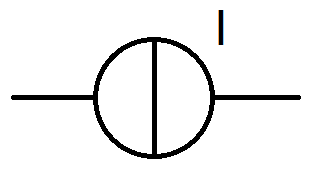
\includegraphics[width=4cm]{pictures/current_source.png}
		\caption{current source symbol}
	\end{figure}
	%\item Diode - to be filled with information after the rest is complete
	%\item Transistor - unlike the other components which were all two-teminal components a transisstor is a three-terminal component
\end{itemize}

The resistance $R$, conductance $G$, capacitance $C$ and inductance $L$ are respectively described as a scalar constant that relates the edge-current to the edge-voltage. If there are more components of the same kind in one circuit their corresponding constants will usually be collected into a matrix which is also called the same and also denoted by the same letter, respectively. These matrices are then positive definite diagonal matrices.

\section{Modified Nodal Analysis - MNA}
\label{sec:MNA}

%num gew dgl steif n steif - seite 422 \newline
%modelling discr circ prob - seite 19

\cite{ModellingAndDiscretizationOfCircuitProblems} and \cite{NumerikGewöhnlicherDifferentialgleichungen}

To analyse the network further we will rearrange the columns of the reduced incidence matrix $A$ such that is has the block form
\begin{displaymath}
	A = (A_R A_C A_L A_V A_I)
\end{displaymath}
where $A_R$, $A_C$, $A_L$, $A_V$ and $A_I$ include the columns that are related to the resistors, capacitors, coils, voltage sources and current sources, respectively.

To mathematically describe the circuit we will use \emph{modified nodal analysis} (or short MNA), first introducced in \textbf{reference original paper!!!!!!!!!!!!!!!!!!!, maybe this?}
	
	introduced by ALBERT E. RUEHLI, see paper	
	
	
	 %https://ieeexplore.ieee.org/document/1084079}. MNA uses the node voltages as well as the currents of the coils and the voltage sources as unknowns. It is based on the conservation laws \eqref{KCL} and \eqref{KVL} as well as on the voltage-current relations of the electrical components, discussed in Section \ref{Sec:Electrical Components and their relation}. The voltages can be represented using the node-potentials
\begin{displaymath}
	v = A^\top u
\end{displaymath}

The vector $v$ can thus be rearranged into $v = (v_R, v_C, v_L, v_{src}, v_I)$. In a similar way we also rearrange the current vector into $i = (i_R, i_C, i_L, i_V, i_src)$. Using the sorted incidence matrix blocks we can rewrite the resistor current relation as
	\begin{displaymath}
		i_R = G \ v_R = G \ A_R^\top u.
	\end{displaymath}
Analogously, we rewrite the capacitor relation as
	\begin{displaymath}
		i_C = C \ v'_C = C \ A_C^\top u'.
	\end{displaymath}

Kirchhoffs current law \eqref{KCL} gives us that
\begin{displaymath}
	A_C i_C + A_R i_R + A_L i_L + A_V i_V = -A_I i_{src}.
\end{displaymath}

We plug in the component relations derived above and obtain
\begin{displaymath}
	A_C C A_C^\top u' + A_R G A_R^\top u + A_L i_L + A_V i_V = -A_I i_{src}.
 \end{displaymath}

Combining this with the component law for inductors \eqref{eq:inductor law} and the potential-voltage relation for voltage sources \eqref{eq:voltage source law} we finally get the modified nodal analysis equations
\begin{displaymath}
	\begin{aligned}
		A_C C A_C^\top u' + A_R G A_R^\top u + A_L i_L + A_V i_V &= - A_I i_{src} , \\
		L i_L'	- A_L^\top u &= 0 , \\
		-A_V^\top u &=  -v_{src}.
	\end{aligned}	
\end{displaymath}

In matrix form these read
\begin{equation}
	\label{MNA_Matrixform}
	\begin{pmatrix}
		A_C C A_C^\top & 0 & 0 \\
		0 & L & 0 \\
		0 & 0 & 0
	\end{pmatrix}
	*
	\begin{pmatrix}
		u' \\
		i_L' \\
		i_V'
	\end{pmatrix}
	+
	\begin{pmatrix}
		A_R G A_R^\top & A_L & A_V \\
		-A_L^\top & 0 & 0 \\
		-A_V^\top & 0 & 0 
	\end{pmatrix}
	*
	\begin{pmatrix}
		u \\
		i_L \\
		i_V
	\end{pmatrix}
	=
	\begin{pmatrix}
		-A_I i_{src} \\
		0 \\
		-v_{src}
	\end{pmatrix} , 
\end{equation}
where the diagonal matrices $C$, $G$ and $L$ contain the capacities, conductivities and inductivities.

The resulting systems are \emph{stiff} systems. This means that for their numerical solution special care has to be put into which methods are suitable for solving these systems in a stable manner.


\textbf{Example 1} \label{ex:MNA} \\
We again consider the charging of a capacitor. The circuit is again given as in Example 1, \ref{ex:network topology}, where we have already derived the reduced incidence matrix
\begin{displaymath}
	A = 
	\left(
	\begin{matrix}
		-1 & 1 & 0 \\
		0 & -1 & 1 
	\end{matrix}
	\right).
\end{displaymath} 
 This matrix can be split into the three submatrices $A_V$, $A_R$ and $A_C$ containing the columns of the matrix $A$. The matrices $A_L$ and $A_V$ are empty in this case. The diagonal matrices containing the components constants are
 \begin{displaymath}
 	C = (C), \qquad L = (), \qquad G = (\frac{1}{R}).
 \end{displaymath}
Plugging this into the formula \eqref{MNA_Matrixform} we obtain the system
\begin{displaymath}
	\begin{pmatrix}
		0 & 0 & 0 \\
		0 & C & 0 \\
		0 & 0 & 0
	\end{pmatrix}
	*
	\begin{pmatrix}
		u_1' \\
		u_2' \\
		i_0'
	\end{pmatrix}
	+
	\begin{pmatrix}
		\frac{1}{R} & -\frac{1}{R} & 0 \\
		-\frac{1}{R} & \frac{1}{R} & -1 \\
		0 & -1 & 0 
	\end{pmatrix}
	*
	\begin{pmatrix}
		u_1 \\
		u_2 \\
		i_0
	\end{pmatrix}
	=
	\begin{pmatrix}
		0 \\
		0 \\
		-v_{src}
	\end{pmatrix}.
\end{displaymath}

\textbf{Example 2} \label{ex:LC-circuit MNA} \\
Similarly we also derived the incidence Matrix of \ref{circuit:LC-circuit} in Example 2, \eqref{ex:LC-circuit incidence matrix}.
\begin{displaymath}
	A = 
	\left(
	\begin{matrix}
		-1 & 1  
	\end{matrix}
	\right).
\end{displaymath}

 This matrix can be split into the two submatrices $A_C$ and $A_L$ containing the columns of the matrix $A$. The matrices $A_R$, $A_V$ and $A_I$ are empty in this case. The diagonal matrices containing the components constants are
\begin{displaymath}
	C = (C), \qquad L = (L).
\end{displaymath}
Plugging this into the formula \eqref{MNA_Matrixform} we obtain the system
\begin{displaymath}
	\begin{pmatrix}
		C & 0 \\
		0 & L 
	\end{pmatrix}
	*
	\begin{pmatrix}
		u_1' \\
		i_L'
	\end{pmatrix}
	+
	\begin{pmatrix}
		0 & 1 \\
		-1 & 0
	\end{pmatrix}
	*
	\begin{pmatrix}
		u_1 \\
		i_L
	\end{pmatrix}
	=
	\begin{pmatrix}
		0 \\
		0 
	\end{pmatrix}.
\end{displaymath}


\textbf{Example 3} \label{ex:Example 3 - MNA} \\
We again consider Example 3, \ref{ex:Example 3 - incidence matrix }. We have already found the incidence matrix for this circuit.
\begin{displaymath}
	A = 
	\left(
	\begin{matrix}
		-1 & 1 & 1
	\end{matrix}
	\right).
\end{displaymath} 
This matrix can be split into the three submatrices $A_I$, $A_R$ and $A_C$ containing the columns of the matrix $A$. The matrices $A_L$ and $A_V$ are empty in this case. The diagonal matrices containing the components constants are
\begin{displaymath}
	C = (C), \qquad L = (), \qquad G = (\frac{1}{R}).
\end{displaymath}
Plugging this into the formula \eqref{MNA_Matrixform} we obtain the system
\begin{displaymath}
	\begin{pmatrix}
		C & 0 \\
		0 & 0 
	\end{pmatrix}
	*
	\begin{pmatrix}
		u_1' \\
		i_V'
	\end{pmatrix}
	+
	\begin{pmatrix}
		\frac{1}{R} & -1 \\
		1 & 0
	\end{pmatrix}
	*
	\begin{pmatrix}
		u_1 \\
		i_V
	\end{pmatrix}
	=
	\begin{pmatrix}
		0 \\
		-v_{src}
	\end{pmatrix}.
\end{displaymath}



%\section{Charge-Flux oriented formulation of MNA}
%\label{sec:charge flux oriented formulation}
% This time we derive the charge and flux based formulations. We again use the KCL \eqref{KCL} and the component equations to formulate a system of equations. This means that instead of directly using current and voltage, we instead use the flux of the magnetic field \eqref{eq:inductor law} and the charge \eqref{eq:capacitor law}. We then obtain
%
%\begin{align}
%	A_C q' + A_R r(A_R^\top u,t) + A_L i_L + A_V i_V + A_I i(A^\top u, q', i_L, i_V, t) &= 0, \label{charge/flux-1} \\
%	\phi' - A_L^\top u &= 0, \label{charge/flux-2} \\
%	v(A^\top u, q', i_L, i_V, t) - A_V^\top u &= 0, \label{charge/flux-3} \\
%	q - q_C(A_C^\top u) &= 0, \label{charge/flux-4} \\
%	\phi - \phi_L(i_L) &= 0.  \label{charge/flux-5} 
%\end{align}
%
%Using node potentials $u$, branch currents through voltage and flux controlled elements $i_V$ and $i_L$, charges and fluxes $q$ and $\phi$, voltage dependent resistors $r$, voltage and current dependent charge and flux sources $q_C$ and $\phi_L$, controlled current and voltage sources $i_{src}$ and $v_{src}$.
%
%We call this formulation the \emph{charge-flux oriented modified nodal analysis}.
%
%%so it makes sense to use the conventional approach of MNA - compare with phd thesis 